\chapter{El grupo fundamental}

\section{Homotopía por arcos}

\begin{definicion}
    Sean $X$ e $Y$ dos espacios topologicos y $f,g:X\to Y$ dos aplicaciones continuas. Decimos que $f$ es \textbf{homotópica} a $g$ si existe $H:X\times[0,1]\to Y$ continua tal que 
    \begin{gather*}
        H(x,0) = f(x) \hspace{0.5cm} \text{ y } \hspace{0.5cm} H(x,1) = g(x) \ \ \ \forall x\in X
    \end{gather*}

    \begin{figure}[H]
        \centering
        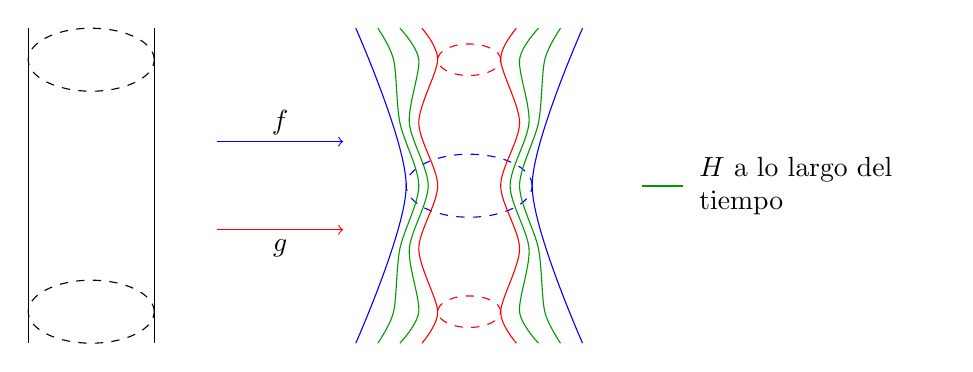
\begin{tikzpicture}[scale=0.8]
            \shorthandoff{>}

            % Cilindro 
            \draw[dashed] (-3,2) ellipse (1 and 0.5);
            \draw[dashed] (-3,-2) ellipse (1 and 0.5);
            \draw (-4,-2.5) -- (-4,2.5);
            \draw (-2,-2.5) -- (-2,2.5);

            % Flecha f
            \node at (0,1) {$f$};
            \draw[->, blue] (-1,0.7) -- (1,0.7);

            % Flecha g
            \node at (0,-1) {$g$};
            \draw[->, red] (-1,-0.7) -- (1,-0.7);

            % Leyenda H
            \node[text width=3cm, anchor=west] at (6.5,0) {$H$ a lo largo del tiempo};
            \draw[thick, green!60!black] (5.75,0)--(6.4,0);

            % Imagen de f
            \draw[dashed, blue] (3,0) ellipse (1 and 0.5);
            \draw[blue] plot[smooth] coordinates {
                (1.2,-2.5) (2,0) (1.2,2.5)
            };
            \draw[blue] plot[smooth] coordinates {
                (4.8,-2.5) (4,0) (4.8,2.5)
            };

            % Imagen de g
            \draw[dashed, red] (3,2) ellipse (0.5 and 0.25);
            \draw[dashed, red] (3,-2) ellipse (0.5 and 0.25);
            \draw[red] plot[smooth] coordinates {
                (2.25,2.5) (2.5,2) (2.2,1) (2.5,0) (2.2,-1) (2.5,-2) (2.25,-2.5)
            };
            \draw[red] plot[smooth] coordinates {
                (3.75,2.5) (3.5,2) (3.8,1) (3.5,0) (3.8,-1) (3.5,-2) (3.75,-2.5)
            };

            % Intermedios derecha
            \draw[green!60!black] plot[smooth] coordinates {
                (4.1,2.5) (3.8,2) (3.95,1) (3.65,0) (3.95,-1) (3.8,-2) (4.1,-2.5)
            };
            \draw[green!60!black] plot[smooth] coordinates {
                (4.45,2.5) (4.2,2) (4.1,1) (3.8,0) (4.1,-1) (4.2,-2) (4.45,-2.5)
            };

            % Intermedios izquierda
            \draw[green!60!black] plot[smooth] coordinates {
                (1.9,2.5) (2.2,2) (2.05,1) (2.35,0) (2.05,-1) (2.2,-2) (1.9,-2.5)
            };
            \draw[green!60!black] plot[smooth] coordinates {
                (1.55,2.5) (1.8,2) (1.9,1) (2.2,0) (1.9,-1) (1.8,-2) (1.55,-2.5)
            };


        \end{tikzpicture}
    \end{figure}

\end{definicion} 

\begin{definicion}
    Dados $X$ e.t., $x,y\in X$ y dos arcos $\alpha, \beta\in \Omega(X;x,y)$, decimos que $\alpha, \beta$ son \textbf{homotópicos por arcos} si existe $H:[0,1]\times [0,1] \to X$ continua tal que 
    \begin{align*}
        H(s,0) = \alpha(s) \hspace{0.5cm} &\text{ y } \hspace{0.5cm} H(s,1) = \beta(x) \ \ \ &\forall s\in [0,1]\\
        H(0,t) = x  \hspace{0.5cm} &\text{ y } \hspace{0.5cm} H(1,t) = y \ \ \ &\forall t \in [0,1]
    \end{align*}
\end{definicion}

\begin{lema}
    Ser homotópico por arcos da lugar a una relación de equivalencia en $\Omega(X;x,y)$.

    \begin{figure}[H]
        \centering
        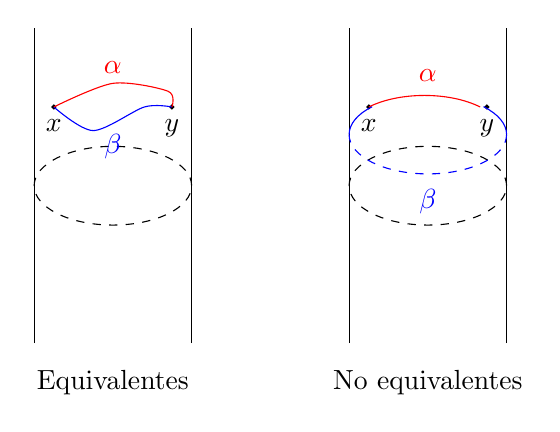
\begin{tikzpicture}
            \shorthandoff{>}

            % Cilindro 1
            \draw[dashed] (-3,0) ellipse (1 and 0.5);
            \draw (-4,-2) -- (-4,2);
            \draw (-2,-2) -- (-2,2);

            % Cilindro 2
            \draw[dashed] (1,0) ellipse (1 and 0.5);
            \draw (0,-2) -- (0,2);
            \draw (2,-2) -- (2,2);

            % Puntos x e y (1)
            \node[draw, circle, fill=black, inner sep=0.5pt, label=below:$x$] at (-3.75,1) {};
            \node[draw, circle, fill=black, inner sep=0.5pt, label=below:$y$] at (-2.25,1) {};

            % Arcos (1)
            \draw[blue] plot[smooth] coordinates {
                (-3.75,1) (-3.25,0.7) (-2.6,1)  (-2.25,1)
            };
            \draw[red] plot[smooth] coordinates {
                (-3.75,1) (-3,1.3) (-2.3,1.2)  (-2.25,1)
            };
            \node[red] at (-3,1.5) {$\alpha$};
            \node[blue] at (-3,0.5) {$\beta$};

            % Puntos x e y (2)
            \node[draw, circle, fill=black, inner sep=0.5pt, label=below:$y$] at (1.75,1) {};
            \node[draw, circle, fill=black, inner sep=0.5pt, label=below:$x$] at (0.25,1) {};

            % Arcos (2)
            \draw[blue, dashed] (2,0.65) arc (0:-180:1 and 0.5);
            \draw[blue] (2,0.65) arc (0:45:1 and 0.5);
            \draw[blue] (0,0.65) arc (180:135:1 and 0.5);
            \draw[red] (0.25,1) arc (135:45:1 and 0.5);
            \node[red] at (1,1.4) {$\alpha$};
            \node[blue] at (1,-0.2) {$\beta$};

            % Textos
            \node at (1,-2.5) {No equivalentes};
            \node at (-3,-2.5) {Equivalentes};

        \end{tikzpicture}
    \end{figure}

    \begin{proof}\
        \begin{enumerate}
            \item[(i)] Dado $\alpha \in \Omega(X;x,y)$ queremos ver que $\alpha$ es homotópica por arcos con $\alpha$. Para ello tenemos 
            \begin{align*}
                H(s,t) = \alpha(s) \hspace{1cm} & H(s,0) = \alpha(s)=H(s,1)\\
                H(0,t) = \alpha(0)=x \hspace{1cm} & H(1,t) = \alpha(1) = y
            \end{align*}

            \item[(ii)] Dados $\alpha, \beta\in \Omega(X;x,y)$ tales que existe $H:[0,1]\times [0,1]\to X$ continua tal que 
            \begin{align*}
                H(s,0) = \alpha(s) \hspace{0.5cm} &\text{ y } \hspace{0.5cm} H(s,1) = \beta(x) \ \ \ &\forall s\in [0,1]\\
                H(0,t) = x  \hspace{0.5cm} &\text{ y } \hspace{0.5cm} H(1,t) = y \ \ \ &\forall t \in [0,1]
            \end{align*}
            Queremos ver que existe un $\tilde{H}:[0,1]\times[0,1]\to X$ continua tal que 
            \begin{align*}
                \tilde{H}(s,0) = \beta(s) \hspace{0.5cm} &\text{ y } \hspace{0.5cm} \tilde{H}(s,1) = \alpha(x) \ \ \ &\forall s\in [0,1]\\
                \tilde{H}(0,t) = x  \hspace{0.5cm} &\text{ y } \hspace{0.5cm} \tilde{H}(1,t) = y \ \ \ &\forall t \in [0,1]
            \end{align*}
            Tomando $\tilde{H}(s,t):=H(s, 1-t)$ cumple claramente con lo que buscamos.

            \item[(iii)] Dado $\alpha, \beta, \gamma\in \Omega(X;x,y)$ y $H_1,H_2:[0,1]\times[0,1]\to X$ continuas tales que 
            \begin{gather*}
                \begin{array}{c c c c}
                    H_1(s,0) = \alpha(s) &&& H_2(s,0) = \beta(s)\\
                    H_1(s,1) = \beta(s) &&& H_2(s,1) = \gamma(s)\\
                    H_1(0,t) = x &&& H_2(0,t) = x\\
                    H_1(1, t) = x &&& H_2(1,t) = y
                \end{array}
            \end{gather*}
            Queremos ver que existe un $H:[0,1]\times [0,1]\to X$ tal que 
            \begin{align*}
                H(s,t) = \alpha(s) \hspace{1cm} & H(s,0) = \alpha(s)=H(s,1)\\
                H(0,t) = \alpha(0)=x \hspace{1cm} & H(1,t) = \alpha(1) = y
            \end{align*}
            Para ello consideramos 
            \begin{gather*}
                H(s,t) = \left\{
                    \begin{array}{l c c}
                        H_1(s,2t) & \text{ si } & 0 \leq t \leq \nicefrac{1}{2}\\
                        H_2(s, 2t-1) & \text{ si } & \nicefrac{1}{2} \leq t \leq 1
                    \end{array}
                \right.
            \end{gather*}
            Y con el lema de pegado es fácil ver que es continua y que satisface las condiciones que buscábamos.
        \end{enumerate}
    \end{proof}
\end{lema}

% TODO: Hacer lo mismo pero para homotopía

\begin{ejemplo}\
    \begin{enumerate}
        \item Sean $X$ un e.t. y $f,g:X \to \bb{R}^n$ aplicaciones continuas, entonces vamos a ver que $f$ y $g$ son homotópicas.
        \begin{proof}
            Vamos a definir la aplicación
            \begin{align*}
                H:X\times [0,1]&\to \bb{R}^n\\
                (x,t) & \mapsto (1-t)f(x) + tg(x)
            \end{align*} 
            que es continua y además verifica
            \begin{gather*}
                H(x,0) = f(x) \hspace{2cm} H(x,1) = g(x)
            \end{gather*}
            por lo que tenemos lo que buscábamos.
        \end{proof}
        En el caso particular de que $f=\alpha$ y $g=\beta$ fuesen arcos comenzando en un punto común y acabando en otro punto común, entonces la $H$ anterior sería una homotopía por arcos.

        \item Si $\alpha: [0,1]\to X$ es un arco y $h:[0,1] \to [0,1]$ es una aplicación continua con $h(0)=0$ y $h(1)=1$, entonces $\dot{\alpha}(s) = \alpha(h(s))$ es homotópica por arcos a $\alpha(s)$.
        
        \begin{proof}
            Es claro que $\dot{\alpha}$ es continua y existe una homotopía por arcos entre $\alpha$ y $\dot{\alpha}$ que es la siguiente
            \begin{gather*}
                H(s,t) = \alpha((1-t)s + th(s))
            \end{gather*}
            que es claramente continua y que verifica que 
            \begin{align*}
                H(s,0) = \alpha(s) \hspace{1cm} & H(s,1) = \alpha(h(s)) = \dot{\alpha}(s)\\
                H(0,t) = \alpha(0)=\dot{\alpha}(1) \hspace{1cm} & H(1,t) = \alpha(1) = \dot{\alpha}(1)
            \end{align*}
        \end{proof}
        Intuitivamente podemos entender esto como que no importa a qué velocidad se recorra una curva para ser homotópico por arcos.
    \end{enumerate} 
\end{ejemplo}

\begin{notacion}
    Como convenio a la clase de equivalencia de un arco $\alpha$ en $\Omega(X;x,y)$ lo denotaremos por $[\alpha]$.
\end{notacion}

\begin{lema}
    Dados dos arcos $\alpha_1, \alpha_2$ en $\Omega(X;x,y)$ y $\beta_1, \beta_2\in \Omega(X; y,z)$. Se verifica que si $[\alpha_1] = [\alpha_2]$, entonces $[\alpha_1\ast\beta_1] = [\alpha_2\ast\beta_2]$.

    \begin{proof}
        Tenemos que 
        \begin{gather*}
            (\alpha_1\ast\beta_1) = \left\{
                \begin{array}{l c c}
                    \alpha_1(2s) & \text{ si } & 0 \leq s \leq \nicefrac{1}{2}\\
                    \beta_1(2s-1) & \text{ si } & \nicefrac{1}{2} \leq s \leq 1
                \end{array}
            \right.\\\\
            (\alpha_2\ast\beta_2) = \left\{
                \begin{array}{l c c}
                    \alpha_2(2s) & \text{ si } & 0 \leq s \leq \nicefrac{1}{2}\\
                    \beta_2(2s-1) & \text{ si } & \nicefrac{1}{2} \leq s \leq 1
                \end{array}
            \right.
        \end{gather*}
        Además, sabemos que existen $H_1, H_2$ continuas tal que 
        \begin{gather*}
            \begin{array}{c c c c}
                H_1(s,0) = \alpha_1(s) &&& H_2(s,0) = \beta_1(s)\\
                H_1(s,1) = \beta_1(s) &&& H_2(s,1) = \beta_2(s)\\
                H_1(0,t) = x &&& H_2(0,t) = y\\
                H_1(1, t) = y &&& H_2(1,t) = z
            \end{array}
        \end{gather*}
        Tomamos entonces $H:[0,1]\times [0,1] \to X$ dada por 
        \begin{gather*}
            H(s,t) = \left\{
                \begin{array}{l c c}
                    H_1(2s, t) & \text{ si } & s \in [0,\nicefrac{1}{2}],\ t\in [0,1]\\
                    H_2(2s-1, t) & \text{ si } & s \in [\nicefrac{1}{2},1],\ t\in [0,1]\\
                \end{array}
            \right.
        \end{gather*}
        es continua y tenemos que 
        \begin{gather*}
            H(s,0) = \left\{
                \begin{array}{l c c}
                    H_1(2s, 0) & \text{ si } & s \in [0,\nicefrac{1}{2}]\\
                    H_2(2s-1, 0) & \text{ si } & s \in [\nicefrac{1}{2},1]\\
                \end{array}
            \right. = 
            \left\{
                \begin{array}{l c c}
                    \alpha_1(2s) & \text{ si } & s \in [0,\nicefrac{1}{2}]\\
                    \beta_1(2s-1) & \text{ si } & s \in [\nicefrac{1}{2},1]\\
                \end{array}
            \right. = (\alpha_1 \ast \beta_1)(s)
        \end{gather*}
        Análogamente se tiene que $H(s,1)=(\alpha_2\ast\beta_2)(s)$ con $H(0,t) = x$ y $H(1,t) = z$.

    \end{proof}
    A partir del lema anterior podemos definir
    \begin{gather*}
        [\alpha] \ast [\beta] := [\alpha \ast \beta]
    \end{gather*}
    con $\alpha\in \Omega(X;x,y)$, $\beta \in \Omega(X;y,z)$
\end{lema}

\begin{teo}
    Dado $X$ e.t., $\alpha\in \Omega(X;x,y)$, $\beta\in \Omega(X;y,z)$ y $\gamma\in \Omega(X;z,w)$ se tiene que 
    \begin{enumerate}
        \item[(i)] $[\alpha] \ast ([\beta] \ast [\gamma]) = ([\alpha] \ast [\beta]) \ast [\gamma]$
        \item[(ii)] $[\alpha]\ast [\veps_y] = [\alpha]$ y $[\veps_x]\ast [\alpha] = [\alpha]$
        \item[(iii)]  $[\alpha]\ast [\tilde{\alpha}] = [\veps_x]$ y $[\tilde{\alpha}]\ast [\alpha] = [\veps_y]$
    \end{enumerate}
    \begin{proof}\
        \begin{enumerate}
            \item[(i)] Desarrollemos cada expresión
            \begin{figure}[H]
                \centering
                \begin{tikzpicture}
                    \shorthandoff{>}

                    % Líneas discontinuas
                    \draw[gray!50, dashed] (0,-1) -- (0,2);
                    \draw[gray!50, dashed] (4,-1) -- (4,2);
                    \draw[gray!50, dashed] (8,-1) -- (8,2);
                    \draw[gray!50, dashed] (12,-1) -- (12,2);
                    
                    % Puntos
                    \node[draw, circle, fill=black, inner sep=0.5pt, label=below:$x$] at (0,0) {};
                    \node[draw, circle, fill=black, inner sep=0.5pt, label=below:$y$] at (4,1) {};
                    \node[draw, circle, fill=black, inner sep=0.5pt, label=below:$z$] at (8,0.8) {};
                    \node[draw, circle, fill=black, inner sep=0.5pt, label=below:$w$] at (12,1) {};

                    % Arcos
                    \draw[blue] plot[smooth, tension=1] coordinates {
                        (0,0) (2,1) (4,1)
                    };
                    \draw[red] plot[smooth, tension=1] coordinates {
                        (4,1) (6,0.6) (8,0.8)
                    };
                    \draw[green!60!black] plot[smooth, tension=1] coordinates {
                        (8,0.8) (9,1) (10.6,0.6) (12,1)
                    };

                    % Nombre arcos
                    \node[blue] at (2,1.3) {$\alpha$};
                    \node[red] at (6,0.9) {$\beta$};
                    \node[green!60!black] at (10,1) {$\gamma$};

                    % Leyenda tiempos
                    \node at (0,-1.2) {$s=0$};
                    \node[violet] at (4,-1.2) {$s=\nicefrac{1}{4}$};
                    \node[violet] at (8,-1.2) {$s=\nicefrac{1}{2}$};
                    \node[orange!90!black] at (4,-1.7) {$s=\nicefrac{1}{2}$};
                    \node[orange!90!black] at (8,-1.7) {$s=\nicefrac{3}{4}$};
                    \node at (12,-1.2) {$s=1$};

                    % Leyenda colores
                    \draw[violet] (13,2)--(13.5,2);
                    \draw[orange!90!black] (13,0)--(13.5,0);
                    \node[anchor=west, text width=2.2cm, align=center] at (13.7,2) {Tiempos de \\$(\alpha\ast\beta)\ast\gamma$};
                    \node[anchor=west, text width=2.2cm, align=center] at (13.7,0) {Tiempos de \\$\alpha\ast(\beta\ast\gamma)$};

                \end{tikzpicture}
            \end{figure}
            \begin{align*}
                (\beta\ast\gamma)(s) &= \left\{
                    \begin{array}{l c c}
                        \beta(2s) & \text{ si } & s \in [0,\nicefrac{1}{2}]\\
                        \gamma(2s-1) & \text{ si } & s \in [\nicefrac{1}{2},1]\\
                    \end{array}
                \right.\\\\
                \alpha \ast(\beta\ast\gamma)(s) &= \left\{
                    \begin{array}{l c c}
                        \alpha(2s) & \text{ si } & s \in [0,\nicefrac{1}{2}]\\
                        (\beta\ast\gamma)(2s-1) & \text{ si } & s \in [\nicefrac{1}{2},1]\\
                    \end{array}
                \right. =\\
                &= \left\{
                    \begin{array}{l c c}
                        \alpha(2s) & \text{ si } & s \in [0,\nicefrac{1}{2}]\\
                        \beta(2(2s-1)) & \text{ si } & s \in [\nicefrac{1}{2},\nicefrac{3}{4}]\\
                        \gamma(2(2s-1)-1) & \text{ si } & s \in [\nicefrac{3}{4},1]\\
                    \end{array}
                \right. = \left\{
                    \begin{array}{l c c}
                        \alpha(2s) & \text{ si } & s \in [0,\nicefrac{1}{2}]\\
                        \beta(4s-2) & \text{ si } & s \in [\nicefrac{1}{2},\nicefrac{3}{4}]\\
                        \gamma(4s-3) & \text{ si } & s \in [\nicefrac{3}{4},1]\\
                    \end{array}
                \right.\\\\\\
                %
                %
                %
                (\alpha\ast\beta)(s) &= \left\{
                    \begin{array}{l c c}
                        \alpha(2s) & \text{ si } & s \in [0,\nicefrac{1}{2}]\\
                        \beta(2s-1) & \text{ si } & s \in [\nicefrac{1}{2},1]\\
                    \end{array}
                \right.\\\\
                (\alpha \ast\beta)\ast\gamma(s) &= \left\{
                    \begin{array}{l c c}
                        (\alpha\ast\beta)(2s) & \text{ si } & s \in [0,\nicefrac{1}{2}]\\
                        \gamma(2s-1) & \text{ si } & s \in [\nicefrac{1}{2},1]\\
                    \end{array}
                \right. =\\
                &= \left\{
                    \begin{array}{l c c}
                        \alpha(2(2s)) & \text{ si } & s \in [0,\nicefrac{1}{4}]\\
                        \beta(2(2s)-1) & \text{ si } & s \in [\nicefrac{1}{4},\nicefrac{1}{2}]\\
                        \gamma(2s-1) & \text{ si } & s \in [\nicefrac{3}{4},1]\\
                    \end{array}
                \right. = \left\{
                    \begin{array}{l c c}
                        \alpha(4s) & \text{ si } & s \in [0,\nicefrac{1}{4}]\\
                        \beta(4s-1) & \text{ si } & s \in [\nicefrac{1}{4},\nicefrac{1}{2}]\\
                        \gamma(2s-1) & \text{ si } & s \in [\nicefrac{1}{2},1]\\
                    \end{array}
                \right.
            \end{align*}

            Usando el ejemplo 2 anterior se tiene que $[\alpha] \ast ([\beta] \ast [\gamma]) = ([\alpha] \ast [\beta]) \ast [\gamma]$ (realmente se están recorriendo las mismas curvas pero a distinta velocidad).


            \item[(ii)] Tendremos que ver que $\alpha \ast \veps_y$ se relaciona por una homotopía con arcos con $\alpha$. Recordemos que
            \begin{gather*}
                (\alpha \ast \veps_y) = \left\{
                    \begin{array}{l c c}
                        \alpha(2s) & \text{ si } & 0\leq s \leq \nicefrac{1}{2} \\
                        \veps_y(2s-1) & \text{ si } & \nicefrac{1}{2} \leq s \leq 1
                    \end{array}
                \right. = 
                \left\{
                    \begin{array}{l c c}
                        \alpha(2s) & \text{ si } & 0\leq s \leq \nicefrac{1}{2} \\
                        y & \text{ si } & \nicefrac{1}{2} \leq s \leq 1
                    \end{array}
                \right.
            \end{gather*}
            De nuevo del ejemplo 2 se tiene que son homotópicas

            \item[(iii)] Tendremos que ver en este caso que $\alpha\ast\tilde{\alpha}$ es homotópico por arcos a $\veps_x$. Describamos ambas curvas.
            \begin{gather*}
                (\alpha \ast \tilde{\alpha}) = \left\{
                    \begin{array}{l c c}
                        \alpha(2s) & \text{ si } & 0\leq s \leq \nicefrac{1}{2} \\
                        \tilde{\alpha}(2s-1) & \text{ si } & \nicefrac{1}{2} \leq s \leq 1
                    \end{array}
                \right. = \left\{
                    \begin{array}{l c c}
                        \alpha(2s) & \text{ si } & 0\leq s \leq \nicefrac{1}{2} \\
                        \tilde{\alpha}(2-2s) & \text{ si } & \nicefrac{1}{2} \leq s \leq 1
                    \end{array}
                \right.\\\\
                \veps_x(s) = x \ \ \ \forall s \in [0,1]
            \end{gather*}
            Pensamos ahora una transformación $H$ que haga que cada vez la curva se vaya quedando más cerca de $x$ (cada vez vuelve antes de llegar a $y$). Intuitivamente podríamos pensar en la siguiente gráfica, en la que vamos reduciendo la distancia desde la función roja hasta la verde
            \begin{figure}[H]
                \centering
                \begin{tikzpicture}[scale=0.75]
                    \begin{axis}[
                        axis lines=left,
                        height=8cm, width=10cm,
                        xmin=-0.2, xmax=1.2,
                        ymin=-0.2, ymax=1.2,
                        xtick={0,0.5,1},
                        ytick={0,1},
                        xticklabels={$0$, $\tfrac{1}{2}$, $1$},
                        yticklabels={$0$,$1$},
                        grid=major,
                        axis x line=middle, % eje X en y=0
                        axis y line=middle, % eje Y en x=0
                        xlabel={$s$},       % nombre eje X
                        ylabel={$t$},       % nombre eje Y
                        xlabel style={below},  % opcional: ajustar posición
                        ylabel style={left},  % opcional: ajustar posición
                    ]
                        % Líneas
                        \addplot[very thick,red!60!black] coordinates {(0,0) (0.5,1) (1,0)};
                        \addplot[very thick,blue!60!black] coordinates {(0,0) (0.5,0.8) (1,0)};
                        \addplot[very thick,yellow] coordinates {(0,0) (0.5,0.3) (1,0)};
                        \addplot[very thick,green!60!black] coordinates {(0,0.01) (0.5,0.01) (1,0.01)};
                    \end{axis}
                \end{tikzpicture}%
            \end{figure}%
            \begin{gather*}
                h(s) = \left\{
                    \begin{array}{l c c}
                        2s & \text{ si } & s\in [0,\nicefrac{1}{2}]\\
                        2-2s & \text{ si } & s\in [\nicefrac{1}{2}, 1]
                    \end{array}
                \right. 
            \end{gather*}
            Y podemos construir $H(s,t) = \alpha((1-t)h(s))$ que claramente es continua y verifica
            \begin{align*}
                H(s,0) = \alpha(h(s)) = (\alpha\ast\tilde{\alpha}(s)) \hspace{0.5cm} &\text{ y } \hspace{0.5cm} H(s,1) = \alpha(0) = x = \veps_x(s) \ \ \ &\forall s\in [0,1]\\
                H(0,t) = \alpha(0) = x  \hspace{0.5cm} &\text{ y } \hspace{0.5cm} H(1,t) = \alpha(0) = x \ \ \ &\forall t \in [0,1]
            \end{align*}
        \end{enumerate}
    \end{proof}

    \section{El grupo fundamental}
    \begin{coro}
        Dados un e.t. $X$ y un punto $x_0\in X$ se tiene que el conjunto de lazos en $X$ basados en $x_0$ bajo la relación de equivalencia de ser homotópicos por arcos y con operación $\ast$ forman un grupo algebraico.

        \begin{proof}
            Definimos el siguiente conjunto
            \begin{gather*}
                G = \frac{\Omega(X;x_0)}{R}
            \end{gather*}
            donde $R$ es la relación de equivalencia ``ser homotópico por arcos''. Veamos ahora que $G$ tiene estructura de grupo:
            \begin{enumerate}
                \item \textbf{Propiedad asociativa.} Tendremos que ver que se verifica para cualesquiera $[\alpha],[\beta], [\gamma]\in G$.
                \begin{gather*}
                    [\alpha] \ast ([\beta] \ast [\gamma]) = ([\alpha] \ast [\beta]) \ast [\gamma]
                \end{gather*}
                pero esto lo tenemos claramente del teorema anterior

                \item \textbf{Existencia del elemento neutro.} Por el teorema anterior tenemos que para $x=y=x_0$ se tiene que $[\alpha] \ast [\veps_{x_0}] = [\alpha] = [\veps_{x_0}] \ast [\alpha]$ para cualquier $[\alpha]\in G$ luego tenemos la existencia probada.
                \item \textbf{Existencia del elemento opuesto.} De nuevo usamos el teorema anterior y nos dice que para cualquier $[\alpha]\in G$ se tiene que 
                \begin{gather*}
                    [\alpha] \ast [\tilde{\alpha}] = [\veps_{x_0}] =  [\tilde{\alpha}] \ast [\alpha] 
                \end{gather*}
                y se tiene directamente.
            \end{enumerate}
            Con esto hemos probado finalmente que $G$ es un grupo.
        \end{proof}
    \end{coro}
\end{teo}

\begin{definicion}
    Al grupo algebraico dado por el corolario anterior lo llamaremos el \textbf{grupo fundamental} de $X$ en $x_0$ y lo denotaremos por $\pi_1(X,x_0)$.
\end{definicion}

\begin{ejemplo} Consideramos $\bb{R}^2\setminus \{0,0\}$ y un punto cualquiera $x_0$.

    \begin{figure}[H]
        \centering
        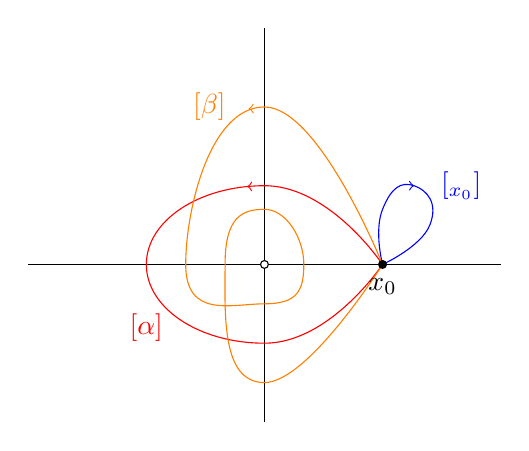
\begin{tikzpicture}
            \shorthandoff{>}

            % Ejes
            \draw (-3,0) -- (3,0);
            \draw (0,-2) -- (0,3);

            % Arcos
            \draw[blue] plot[smooth, tension=1] coordinates {
                (1.5,0) (1.5,0.7) (1.9,1) (2.1,0.5) (1.5,0)
            };
            \draw[->, blue] (1.9,1) ++(-0.01, 0) -- ++(0.01,0);


            \draw[red] plot[smooth, tension=1] coordinates {
                (1.5,0) (0,1) (-1.5,0) (0,-1) (1.5,0)
            };
            \draw[->, red] (-0.22,0.99) ++(+0.01, 0) -- ++(-0.01,0);

            \draw[orange] plot[smooth, tension=1] coordinates {
                (1.5,0) (0,2) (-1,0) (0,-0.5) (0.5,0) (0,0.7) (-0.5, 0) (0,-1.5) (1.5,0)
            };
            \draw[->, orange] (-0.2,1.98) ++(+0.01, 0) -- ++(-0.01,0);

            % Leyendas
            \node[blue] at (2.5,1) {$[\veps_{x_0}]$};
            \node[red] at (-1.5, -0.8) {$[\alpha]$};
            \node[orange] at (-0.7, 2) {$[\beta]$};

            % Puntos
            \node[draw, circle, fill=white, inner sep=1pt] at (0,0) {};
            \node[draw, circle, fill=black, inner sep=1pt, label=below:$x_0$] at (1.5,0) {};

        \end{tikzpicture}%
    \end{figure}%

    En este espacio tenemos que $[\veps_{x_0}] \neq [\alpha] \neq [\tilde{\alpha}] \neq [\beta]$. Intuitivamente podríamos intentar identificar este espacio con $\bb{Z}$ de la siguiente forma:
    
    \begin{itemize}
        \item La clase $[\veps_{x_0}]$ la podemos interpretar como el $0$ de $\bb{Z}$.
        \item Identificaremos los números positivos como el número de vueltas que da cada curva al punto $(0,0)$ en sentido positivo (el que elijamos como positivo). Por ejemplo $[\alpha]$ sería $1\in \bb{Z}$, $[\beta]$ sería $2\in \bb{Z}$ y podríamos seguir así con todos los números enteros.
        \item Para los números negativos tomaremos los opuestos de los anteriores, es decir, las curvas recorridas en sentido contrario. Por ejemplo $[\tilde{\alpha}]$ será el $-1\in \bb{Z}$, $[\tilde{\beta}]$ será el $-2$ y así sucesivamente. 
    \end{itemize}

    Más adelante probaremos que $\pi_1(X,x_0)$ es isomorfo a $\bb{Z}$ de una forma más rigurosa.
\end{ejemplo}

\begin{ejemplo}
    Sea $X\subseteq \bb{R}^n$ un subconjunto estrellado desde un punto $x_0$. Entonces $\pi_1(X;x_0) = \{[\veps_{x_0}]\}$, es decir, es trivial.

    \begin{proof}
        Dado $\alpha(s)$ un lazo basado en $x_0$ dentro de $X$, entonces 
        \begin{gather*}
            H(s,t) = (1-t)\alpha(s)+tx_0
        \end{gather*}
        es una aplicación continua dentro\footnote{aquí es donde usamos que es estrellado} de $X$ tal que 
        \begin{align*}
            H(s,0) = \alpha(s) = \hspace{0.5cm} &\text{ y } \hspace{0.5cm} H(s,1) = x_0 = \veps_{x_0}(s) \ \ \ &\forall s\in [0,1]\\
            H(0,t) = x_0  \hspace{0.5cm} &\text{ y } \hspace{0.5cm} H(1,t) = x_0\ \ \ &\forall t \in [0,1]
        \end{align*}
    \end{proof}
    En particular, las bolas abiertas, las bolas cerradas, los convexos en general como $\bb{R}^n$ tienen grupo fundamental trivial.
\end{ejemplo}

\begin{teo}
    Sean $x,y$ dos puntos de un e.t. $X$. Si $X$ es arcoconexo, entonces $\pi_1(X,x)$ y $\pi_1(X,y)$ son iguales salvo isomorfismo.
    \begin{proof}
        Como $X$ es arcoconexo podemos considerar $\alpha$ un arco uniendo $x$ con $y$ y la aplicación
        \begin{align*}
            F_\alpha : \pi_1(X,y) &\to \pi_1(X,x)\\
            [\gamma] & \mapsto [\alpha]\ast[\gamma]\ast[\tilde{\alpha}]
        \end{align*}
        que está bien definida por lo visto anteriormente sobre el operador $\ast$. Queremos ver ahora que $F_\alpha$ es un isomorfismo de grupos. Para ello comencemos por ver que $F_\alpha$ es un homomorfismo, es decir, que se verifica
        \begin{gather*}
            F_\alpha([\gamma_1] \ast [\gamma_2]) = F_\alpha[\gamma_1]\ast F_\alpha([\gamma_2])
        \end{gather*}
        Desarrollamos el segundo término de la expresión:
        \begin{align*}
            F_\alpha[\gamma_1]\ast F_\alpha([\gamma_2]) &= ([\alpha] \ast [\gamma_1] \ast [\tilde{\alpha}]) \ast ([\alpha] \ast [\gamma_2] \ast [\tilde{\alpha}]) = [\alpha] \ast [\gamma_1] \ast [\gamma_2] \ast [\tilde{\alpha}] =\\
            &= F_\alpha([\gamma_1] \ast [\gamma_2])
        \end{align*}
        y tenemos la igualdad buscada. Veamos ahora que tiene inversa considerando $F_{\tilde{\alpha}}$ que por definición es $F_{\tilde{\alpha}}([\beta]) = [\tilde{\alpha}] \ast [\beta] \ast [\alpha]$ y que además verifica
        \begin{gather*}
            (F_{\tilde{\alpha}} \circ F_{\tilde{\alpha}})([\gamma]) = F_{\tilde{\alpha}}([\alpha]\ast [\gamma]\ast [\tilde{\alpha}]) = [\tilde{\alpha}] \ast ([\alpha]\ast [\gamma]\ast [\tilde{\alpha}]) \ast [\alpha] = [\gamma] = Id_{\pi_1(X,y)}([\gamma])\\
            %
            (F_\alpha \circ F_{\tilde{\alpha}})([\gamma]) = F_\alpha([\tilde{\alpha}] \ast [\gamma] \ast [\alpha]) = [\alpha] \ast ([\tilde{\alpha}] \ast [\gamma] \ast [\alpha]) \ast [\tilde{\alpha}] = [\gamma] = Id_{\pi_1(X,x)}([\gamma])
        \end{gather*}
        por lo que es su inversa. Hemos encontrado por tanto un homomorfismo biyectivo, luego $\pi_1(X,x) \cong \pi_1(X,y)$
    \end{proof}
\end{teo}

\begin{definicion}
    Decimos que un e.t. es \textbf{simplemente conexo} si es arcoconexo y su grupo fundamental es el trivial en un punto (y, por tanto, en cualquier punto).
\end{definicion}

\begin{ejemplo}
    Si $A\subset \bb{R}^n$ es estrellado desde un punto $x_0$, entonces $A$ es simplemente conexo.
\end{ejemplo}

\begin{lema}
    Sea $f:X\to Y$ una aplicación continua entre espacios topológicos y $x\in X$. Entonces la aplicación
    \begin{align*}
        (f_x)_* : \pi_1(X,x) &\to \pi_1(Y,f(x))\\
        [\alpha] &\mapsto [f\circ \alpha]
    \end{align*}
    está bien definida y es un homomorfismo de grupos\footnote{Cuando no haya confusión posible escribiremos solamente $f_*$ en lugar de $(f_x)_*$}.

    \begin{proof}
        Para ver que $(f_x)_*$ está bien definida tomamos $\alpha_1,\ \alpha_2$ lazos basados en $x$ tales que $[\alpha_1] = [\alpha_2]$. Queremos comprobar que $[f\circ \alpha_1] = [f\circ \alpha_2]$. Para ello , sabemos que si $[\alpha_1] = [\alpha_2]$, entonces existe $H:[0,1]\to X$ continua y tal que
        \begin{gather*}
            H(s,0) =\alpha_1(s)\ \ \  ,\ \ \ H(s,1) = \alpha_2(s)\ \ \ , \ \ \ H(0,t)=x=H(1,t)
        \end{gather*}
        Entonces podemos considerar la aplicación 
        \begin{align*}
            f\circ H : [0,1]\times [0,1] \to Y
        \end{align*}
        que es continua y verifica 
        \begin{gather*}
            (f\circ H) (s,0) = (f \circ \alpha_1)(s)\\
            (f\circ H) (s,1) = (f\circ \alpha_2)(s)\\
            (f\circ H) (0,t) = f(x) = (f\circ H) (1,t)
        \end{gather*}
        por lo que $[f\circ \alpha_1] = [f\circ \alpha_2]$. Veamos ahora que $(f_x)_*$ es un homomorfismo de grupos, es decir que se verifica
        \begin{gather*}
            (f_x)_* ([\alpha] \ast [\beta] ) = (f_x)_* ([\alpha]) \ast (f_x)_* ([\beta])
        \end{gather*}
        Por definición sabemos que 
        \begin{gather*}
            (f_x)_* ([\alpha] \ast [\beta] ) = (f_x)_*([\alpha \ast \beta]) = [f\circ(\alpha \ast \beta)] = \left[\left\{
                \begin{array}{l c c}
                    f(\alpha(2s)) & \text{ si } & 0\leq s \leq \nicefrac{1}{2}\\
                    f(\beta(2s-1)) & \text{ si } & \nicefrac{1}{2} \leq s \leq 1\\
                \end{array}
            \right.\right]=\\
            =[(f\ast \alpha) \ast (f\circ \beta)] = (f_x)_* ([\alpha]) \ast (f_x)_* ([\beta])
        \end{gather*}
    \end{proof}
\end{lema}

\begin{definicion}
    A la aplicación $f_x$ dada por el lema la llamaremos \textbf{homomorfismo inducido} por $f$.
\end{definicion}

\begin{propiedades}
    Algunas propiedades básicas de $f_x$ son
    \begin{enumerate}
        \item Si tenemos dos aplicaciones continuas $f:X\to Y$ y $g:Y \to Z$, entonces se tiene que 
        \begin{gather*}
            (g\circ f)_* = g_x \circ f_x
        \end{gather*}

        \item  Se verifica que la aplicación dada por
        \begin{align*}
            Id_x: \pi_1(X,x_0) &\to \pi(X,x_0)\\
            [\alpha] & \mapsto [\alpha]
        \end{align*}
        es la identidad en grupos fundamentales.
    \end{enumerate}
\end{propiedades}

\begin{coro}
    Si $h:X\to Y$ es un homeomorfismo, entonces la aplicación dada por
    \begin{gather*}
        (h_x)_*:\pi_1(X,x) \to \pi_1(Y,h(x))
    \end{gather*}
    es un isomorfismo de grupos, es decir, el grupo fundamental se conserva\footnote{salvo isomorfismo} por homeomorfismos.
\end{coro}

\begin{definicion}
    Si $(G_1,\ast_1)$ y $(G_2, \ast_2)$ son dos grupos algebraicos, consideramos sobre $G_1\times G_2$ el producto $\ast$ dado por 
    \begin{gather*}
        (a_1,b_1)\ast(a_2,b_2) := (a_1\ast_1 a_2, b_1 \ast_2 b_2)
    \end{gather*}
    para $a_1,a_2\in G_1$, $b_1,b_2\in G_2$
\end{definicion}

\begin{teo}
    Sean $X,Y$ dos e.t., $x\in X$, $y\in Y$. Entonces, con la topología producto en $X\times Y$ se tiene que 
    \begin{gather*}
        \pi_1(X\times Y, (x,y)) \cong \pi_1(X,x) \times \pi_1(Y,y)
    \end{gather*}
    \begin{proof}
        Veasmos que 
        \begin{align*}
            \phi: \pi_1(X\times Y,(x,y)) &\longrightarrow \pi_1(X,x) \times \pi_1(Y,y) \\
            [\alpha] & \longmapsto ([p_1 \circ \alpha], [p_2\circ \alpha])
        \end{align*}
        donde $p_1$ y $p_2$ son las proyecciones a $X$ y a $Y$ respectivamente está bien definida. Esto es fácil de ver ya que 
        \begin{gather*}
            ([p_1 \circ \alpha], [p_2\circ \alpha]) = ((p_1)_*([\alpha]), (p_2)_*([\alpha]))
        \end{gather*}
        y además es un homomorfismo. Consideramos además la siguiente aplicación
        \begin{align*}
            \psi: \pi_1(X,x)\times \pi_1(Y,y) \longrightarrow \pi_1(X\times Y, (x,y))\\
            ([\beta], [\gamma]) & \longmapsto [(\beta, \gamma)]
        \end{align*}
        y es fácil ver que está bien definida y es un homomorfismo tal que
        \begin{gather*}
            \psi \circ \phi = Id_{\pi_1(X\times Y,(x,y))}\\
            \phi \circ \psi = Id_{\pi_1(X,x) \times \pi_1(Y,y)}
        \end{gather*}
    \end{proof}
\end{teo}

\section{Espacios recubridores}

\begin{definicion}
    Sea $p:R\to B$ una aplicación continua y sobreyectiva entre dos espacios topológicos. Dado un punto $b\in B$ decimos que un abierto $O$ que contiene a $b$ está \textbf{regularmente recubierto} si se verifican las siguientes propiedades
    \begin{enumerate}
        \item $p^{-1}(O)$ es una unión disjunta de abiertos $A_i\subseteq R$, $i\in I$.
        \item Para cada $i\in I$, $p_{|A_i}:A_i \to O$ es un homeomorfismo.
    \end{enumerate}
\end{definicion}

